\documentclass[withoutpreface,bwprint]{cumcmthesis} % 去除承诺书和编号页
\title{校门开放方式对于通行效率的影响探究}

\begin{document}
\maketitle
\begin{abstract}
本文旨在探究校门开放方式对学生通行效率的影响。
通过排队论的方法,建立了三种不同复杂度的模型来分析和比较两种开门模
式:默认开门和默认关门。首先,我们简化了模型,假设非高峰期单校门情
形下的随机服务时间为固定数值,构建了模型1。接着,模型2引入了负指数
分布来更细致地描述服务时间。最后,模型3综合考虑了高峰期和非高峰期,
多校门情形以及顾客流在不同队列中的转移概率,是最符合实际的模型。

为了构建排队论基本模型,对服务规则与顾客源建立随机性模型。
在服务规则分析中,我们考虑了刷卡时间和经过时间的波动性,并采用负
指数分布来描述校门的服务过程。顾客源分析则区分了学生和其他人员,分
别建立了适用于高峰期和非高峰期的泊松流模型。此外,还考虑了步行与单
车两种不同的出行方式,并对刷卡成功率进行了建模。

理论分析部分,我们使用了排队论的基本公式和概率论,得到了描述系统运
行特征的差分方程,然后求得了稳态解,并通过状态转移图的方式进行可视化。
对于不同的模型,分别通过Pollaczek-Khintchine公式
和Little法则,计算了平均队长和平均等待时间,并将数值模拟时
用到的参数代入公式。定性的来说,各模型中均可以表示默认关门的通行效率
要低于默认开门的模式。定量的来说,对于单通道模型下的默认开门的平均队长
与默认关门的平均队长的比值,确定服务型为0.52,随机服务型为0.42.

数值模拟部分,我们采用了元胞自动机模型和蒙特卡洛法,对排队-通行过程进行了精细模拟
,并进行了统计分析以验证理论解的正确性。元胞自动机分别模拟单通道与多通道
的情况,在多通道时,设置转移概率,有效模拟真实过程,并进行可视化展示。
统计结果时,使用10000个时间步长下的平均队列作为评价指标,
模拟100次,对结果进行统计分析,最后在$95\%$的置信度下,
给出两者平均队长之比的置信区间为[0.4516,0.4526],与理论结果的定性结果一致,
在具体的定量分析上有有一定差距。
\par 考虑实际情况,在单通道随机模型的基础上建立多通道随机模型,重要的特征是
行人可以以一定的概率换道,从而更快的通过校门。在高人流量和低人流量的情况下分别对
单通道和多通道模型进行数值模拟,得到平均队长。模拟结果显示,多通道可以显著减少
平均队长,同时在多通道、成功率较高的情况下,两种开门方式下的通行效率相差不大。
考虑到校园管理对于安全性的需求,结合模拟结果,给出不同场景下的开门方式建议。
\par 最后,在模型建立完成的基础上对模型进行评价与展望。
本文讨论了模型的优缺点,并提出了改进方向,包括实地调研获取参数、选择更
符合实际的模型以及将模型推广到更多场景。

\keywords{排队论\quad 通行方式 \quad 元胞自动机 \quad 泊松过程}
\end{abstract}
\section{问题分析}
\subsection{建模基本思路}
从理论的角度,通过排队论的方法对问题进行建模。需要考虑到服务对象,服务规则来构建排队模型,使用
常见的系统平均队长$ L_s$,平均等待时间$W_s$,服务强度$\rho$等概念来对比两种开门模式的效率。
另一方面,从模拟的角度,基于理论分析的顾客、服务模型,建立元胞自动机模拟
排队过程,计算最终结果,与理论计算值进行对比。
\par 由于两个开门模式的差别在于服务模式的不同,而对于顾客源,两者是一致的。
因此,可以将顾客源进行适当的简化,而突出服务模式的对排队系统的影响。
\par 另一方面,研究由浅入深,建立三个模型,模型的复杂度逐步增加,效果更加接近实际:
\begin{description}
    \item[模型1] 在时间上,只考虑非高峰期,在通道上只考虑一个校门的情形,在服务系统方面将随机服务时间用
    固定数值(均值)代替,从而简化模型。
    \item[模型2] 在时间上,只考虑非高峰期,在通道上只考虑一个校门的情形,在服务系统方面,随机服务时间用
    负指数分布来描述,从而细化对服务系统的刻画。
    \item[模型3] 在时间上,既考虑非高峰期,又考虑高峰期,在通道上考虑多个校门的情形,并且
    顾客流可以在不同队列中按照一定概率转移,在服务系统方面,随机服务时间用
    负指数分布来描述,得到最终的效率对比结果。
\end{description}
以下对这些问题一一建模。

\subsection{服务规则分析}
	在两种方案中,无论默认状态是开门还是关门,顾客的服务时间都是相对固定的。

    对于默认关门的情况,顺利刷卡的服务时间为刷卡时间$t_{g}$,开门时间$t_{o}$,经过时间$t_{p}$
    与关门时间$t_{c}$组成。其中开门、关门时间即为定值,而且是相等的,
    相加作为固定服务时间$2t_{c}$。而刷卡时间、经过时间有一定的波动,
    对于不同年龄、不同身份、不同交通工具的人有较大的差异。
    例如,骑行单车入校的人由于要控制单车,取出与放回校园卡
    的时间比步行要长;年龄较大的人通过时间比年轻人要长;通过时看手机
    的人,通过时间比正常通行的人要长。将这两个服务时间之和即为随机服务时间$t_{r}$
    
    但总的来说,校门的随机服务时间有一定的共性。首先,服务时间必然是正数;其次大多数人的
    服务时间都较为稳定,服务时间极长的人很少。为了描述这种变化,使用常见的负指数分布
    来描述校门的服务过程。

    最后将固定服务时间与随机服务时间相加即为总服务时间$t_{all}=2t_{c}+t_{r}$.

    而对于刷卡失败的情况,在非高峰期时,队列稀疏的情况下,对正常队列的影响不大,
    但是在高峰期时,由于进出压力大,人们在刷卡的流程中形成惯性,而刷卡失败会
    导致队列结果的破坏与前后人流的拥堵,从而大大降低通过效率,
    甚至导致整条队列的长期停滞。对刷卡失败的情况,需要细致的建模。

    对于默认开门的情况,顺利刷卡的服务时间为刷卡时间与经过时间,也可以视为定值。
    但是对于刷卡失败的人员,需要在保安的协助下进行登记之后才能入内,而下一个
    人的经过时间需要加上开门时间。

\subsection{顾客源分析}
在我们的问题中,服务对象为进出校的学生以及其他人员。在这些服务对象中,又分为步行
与单车两重出行方式。在分布时间上,又分为高峰期与非高峰期。总的来说需要对不同时期、不同方式、
不同身份的服务对象分别进行建模,以下是具体分析过程

\subsubsection{学生}
	学生群体是所有服务对象中规模最大,成分最复杂的情况,也是开门方式能够影响的主要人员,需
    要进行详细的建模。

	从时间分布的角度来说,由于学生群体在高峰期与非高峰期上具有明显的差异。在非高峰期时,学生
    进出校门的时间随机性强,且较为稀疏。进一步分析,在不相互重叠的时间段内顾客到达的数量
    是相互独立的;且在任意时间段内,到达的概率与时间无关,因为在非高峰期的出行没有显著规律;
    最后,由于非高峰期人群的通行具有稀疏性,所以在短时间内有多人进入的概率极小。
    
    综合以上原因,顾客源适合用标准泊松流来建模。而且由于几乎不存在过于拥挤的
    可能,因此也不考虑容量限制。即$M/G/1/\infty/\infty/FCFS$模型。

    在高峰期,人员流动迅速,排队长度较长,但是高峰期的流通人数是由限制的,即顾客源的容
    量是有限的,将此时顾客源的容量记为$C_{source}$。而且在校门口排队的空间容量是有限的,
    在高峰期容易被填满,将此时的总容量记为$C_{queue}$。但总体来说,顾
    客到来的间隔时间还是可以服从一个均值较小的泊松分布,这个均值比非高峰期要小得多。综合
    起来,高峰期的学生进校排队模型可以简化为$M/G/3/C_{queue}/C_{source}/FCFS$
    此外,由于步行与单车在排队是占据的空间有多不同,所以最后的空间限制并非直接作用于人数,
    而是需要通过作用于空间,间接控制人数。

    从刷卡成功率的角度分析,学生群体的刷卡成功率很高。

\subsubsection{其他}
    对于其他人群,在进校时间上没有明显的高峰期与非高峰期之分,所以用统一的泊松过程模拟即可。
    而且由于其他人群的进出校需求与非高峰期的学生大致相当,可以直接与学生统一。
    对于交通方式来说,主要是步行,而骑单车的人数较少,故简化为全步行。
    在刷卡成功率方面,这个群体的成功率要比学生群体更低。如果与学生顾客源
    统一,则需要按照双方人数加权平均,得到综合的刷卡成功率。
\section{符号说明}
\begin{table}[h]
    \small
    \centering
    \caption{符号说明表格}\label{tab:symbols}
    \begin{tabular}{c>{\centering\arraybackslash}p{0.7\textwidth}>
        {\centering\arraybackslash}p{0.1\textwidth}}
        \toprule[1.5pt]
        符号 & 符号说明 & 量纲\\
        \midrule[1pt]
        $ t_g $ & 刷卡时间 & $s$\\
        $ t_o $ & 开门时间 & $s$\\
        $ t_p $ & 经过时间 & $s$\\
        $ t_c $ & 关门时间 & $s$\\
        $ t_s $ & 随机服务时间 & $s$\\
        $ t_{all} $ & 总服务时间 & $s$\\
        $ v_f$ & 队伍前进速度 & $m/s$\\
        $ p_s$ & 换道的概率 & $-$ \\
        $C_{source}$ & 顾客源的容量 & $-$ \\
        $C_{queue}$ & 队列的空间容量 & $-$ \\
        $ l_b$ & 自行车占据空间 & $m$\\
        $ l_p$ & 普通行人占据空间 & $m$\\
        $ L_s$ & 服务系统中的总共人数 & $-$\\
        $ L_q$ & 服务系统队列中的人数 & $-$\\
        $ W_s$ & 服务系统中平均等待时长 & $s$\\
        $ W_q$ & 服务系统队列平均等待时长 & $s$\\
        $ \lambda_l$ & 非高峰期时人群的平均到达率 & $-$\\
        $ \lambda_h$ & 高峰期时人群的平均到达率 & $-$\\
        $ \mu $ & 随机服务时的单位时间内的服务人数 & $-$\\
        $ \rho $ & 服务强度 & $-$\\
        \bottomrule[1.5pt]
    \end{tabular}
\end{table}
\section{模型假设}
\begin{enumerate}
    \setlength{\leftskip}{0pt}
    \item \textbf{服务对象由行人和自行车组成,自行车在排队时会下车推行}。
    \\ 根据实际生活经验,排队人群主要由行人和自行车组成,同时自行车多会下车推行,从而在校门前
    行人和自行车的速度可以认为一致。同时由于自行车和行人占用的空间大小不同,在问题求解过程中将两者
    分开建模。
    \item \textbf{行人在排队时如果发现前方队伍发生阻塞,有一定概率换道,这个概率对所有的行人相同,但是自行车
    不会换道}。
    \\ 行人为了更快通过校门,在发现前方队伍发生阻塞时往往会进行换道。在满足换道条件时(建模过程中
    将会定量说明)会有一定的概率换道。但是自行车由于所占空间较大,往往不会换道,所以这里为了简化模型,
    假设自行车不会换道。
    \item \textbf{刷卡失败后,默认该对象离开队伍,重新排队后刷卡进校}。
    \\ 在行人刷身份证进校时,由于不知道在哪里刷卡,往往会花费较长的刷卡时间,失败的概率也较高。观察到
    这样的行人一般会在安保人员的引导下先离开队伍,等到队伍有空位时再次刷身份证进校。所以如果刷卡失败,假设
    行人会先离开队伍,重新排队后再次刷卡入校。
\end{enumerate}
\section{模型建立与求解}
\subsection{基本理论}
\subsubsection{服务系统的规则设定}
    首先从理论上,基于排队论的基本公式与概率论相关知识,在理论上对两种开门模型
    进行理论计算,得到平均队长与平均等待时间作为评价通行效率的指标。

    从顾客源的角度来说,顾客源的输入为泊松过程,泊松过程的概率表达式如下

    \begin{equation}
        P_n(t)=\frac{e^{-\lambda t}(\lambda t)^n}{n!},t>0,n \in \mathbb{N}
    \end{equation}
    $\lambda$表示单位时间内平均到达的顾客数,
    对于非高峰期与高峰期的顾客源,分别使用不同的$\lambda_l,\lambda_h$来描述。

    按照泊松过程的概率公式,随机生成顾客队列,
    并让队列以$v_f=1 m/s$的速度前进。

    对于到达校门的人,开始进行服务。服务时间由固定服务时间与随机服务时间相加得到,
    即$t_{all}=2t_{c}+t_{r}$。$t_r$服从负指数分布,概率密度与分布函数如下:
    \begin{equation}
        \begin{aligned}
            f(t) &=\mu e^{-\mu t},  \\
            F(t) &=1-e^{-\mu t},t>0
        \end{aligned}
    \end{equation}

    求的随机服务时间$t_r$的数学期望$E(t_r)=\frac{1}{\mu}$即为平均随机服务时间,
    因此$\mu$的意义就是单位时间内的平均服务人数,也就是校门的平均通过速率。
    在加上固定服务时间$2t_c$,得到总服务时间的数学期望$E(t_{all})=2t_c+\frac{1}{\mu}$,
    方差$ Var(t_{all})=Var(t_r)=\frac{1}{\mu^2}$。
    对于精度要求不高的模型,也可以使用一个常数(平均服务时间)来代替,
    即数学期望$E(t_{all})=2t_c+\frac{1}{\mu}$,
    方差$ Var(t_{all})=0$。

    有了顾客源与服务时间的随机分布模型,可以服务定义强度
    $\rho=\lambda E(t_{all})=2t_c \lambda+\frac{\lambda}{\mu}$

    在这里假设服务强度$\rho<1$,而这个假设也是合理的,因为否则会导致队伍长度发散。
    使用排队论中的经典公式Pollaczek-Khintchine公式,对于一个任意分布的服务时间T,
    且规定对应分布的服务强度$\rho=\lambda E(t_{all})$,有
    \begin{equation}
        L_s=\rho +\frac{\rho^2 +\lambda^2 Var(T)}{2(1-\rho)}
    \end{equation}
    根据Little法则,可以对平均服务长度与平均等待时长进行换算
    \begin{equation}
        L_s=\lambda W_s
    \end{equation}

    基于以上理论分析,给出我们模型的理论平均队长与理论平均等待时间,
    在考虑随机服务时间为定值的条件下
    \begin{equation}
        \begin{aligned}
            L_s & =\rho +\frac{\rho^2 }{2(1-\rho)} \\
            W_s &=\frac{\rho}{\lambda} +\frac{\rho^2}{2\lambda (1-\rho)}
        \end{aligned}
    \end{equation}
    在考虑随机服务时间为负指数分布的条件下
    \begin{equation}
        \begin{aligned}
            L_s & =\rho +\frac{\rho^2 +\lambda^2 /\mu^2}{2(1-\rho)} \\
            W_s &=\frac{\rho}{\lambda} +\frac{\rho^2 +\lambda^2 /\mu^2}{2\lambda (1-\rho)}
        \end{aligned}
    \end{equation}

\subsubsection{求解方法}
    为了细致的分析这一过程,我们需要求解得到系统的运行特征$P_n(t)$,
    它表示系统在任意时刻t系统中有n个人的概率。
    
    为方便后续的描述,将平均服务时间简写为$\frac{1}{\mu}$,实际为$2t_c+\frac{1}{\mu}$。
    
    先在t时刻与$t+\Delta t$时刻之间的时间段内进行研究。由于在任意时间段内
    一个顾客到达的概率与t无关,所以有一个顾客到来的概率为$\lambda \Delta t$,
    与之对应,没有顾客到来的概率为$1- \lambda \Delta t$。
    
    由于此时将服务时间简化为定值,所以这段时间内一个顾客离去的概率为$\mu \Delta t$,
    没有顾客离去的概率为$1-\mu \Delta t$。
    
    发生两个以上顾客到来或者离去的概率为以上两个概率的平方,所以是$o(\Delta)t$,可以忽略不计。
    
    接下来,在t时刻与$t+\Delta t$时刻之间的时间段内,可能发生四种情况,
    \begin{itemize}
    \item 一个人到来,一个人离去,概率为$\lambda \Delta t \cdot \mu \Delta t$,结果为人数加1。
    \item 一个人到来,没有人离去,概率为$\lambda \Delta t \cdot (1-\mu \Delta) t$,结果为人数不变。
    \item 没有人到来,一个人离去,概率为$(1-\lambda \Delta) t \cdot \mu \Delta t$,结果为人数减1。
    \item 没有人到来,没有人离去,概率为$(1-\lambda \Delta t) \cdot (1-\mu \Delta) t$,结果为人数不变。
    \end{itemize}
    
    
    再考虑在时刻t时,有n-1,n,n+1个顾客时的情形,要想在时刻$t+\Delta t$时有n个人,
    只有三种情况(不考虑两个人以上的变动),
    \begin{itemize}
    \item 在时刻t有n个人,在接下来$\Delta t$时间段内人数不变。
    \item 在时刻t有n-1个人,在接下来$\Delta t$时间段内人数加1。
    \item 在时刻t有n+1个人,在接下来$\Delta t$时间段内人数减1。 
    \end{itemize}
    
    
    综合得到以下状态转移概率公式:
    \begin{equation}
        P_n(t+\Delta t)=P_n(t)(1-\lambda \Delta t-\mu \Delta t)+P_{n+1}(t)(\mu \Delta t) +P_{n-1}(t)(\lambda \Delta t)+o(\Delta t)
    \end{equation}
    
    在这个状态转移概率公式中对t取极限,得到关于$P_n(t)$差分微分方程:
    \begin{equation}
        \frac{d P_n(t)}{dt}=\lambda P_{n-1}(t)+\mu P_{n+1}(t)-(\lambda+\mu )P_n(t)
    \end{equation}
    
    我们只关心系统状态的稳态解,而不关心系统状态的瞬态解,所以只考虑$P_n$,而不是$P_n(t)$。
    
    从而得到一个关于稳态状态之间的差分方程:
    \begin{equation}
        \begin{aligned}
            \lambda P_{n-1}(t)+\mu P_{n+1}(t)-(\lambda+\mu )P_n(t)&=0,n\geq 1 \\
            -\lambda P_{0}+\mu P_{1}&=0
        \end{aligned}
    \end{equation}
    
    以上的差分方程是很好求解的,由于顾客源于排队的空间都设置为无穷大,所以可以解得:
    \begin{equation}
        \begin{aligned}
            P_0 &=1-\rho \\
            P_n &=(1-\rho)\rho^n,n\geq1
        \end{aligned}
    \end{equation}
    其中的$\rho=\frac{\lambda}{\mu}$,它的物理意义为服务强度。
    
    从而可以得到$L_s$的数学期望$L_s=\frac{\rho}{1-\rho}$,这与
    基本理论中的Pollaczek-Khintchine公式结果是一致的。
\subsection{单通道确定性模型}
\subsubsection{理论分析}
首先考虑非高峰期的情况下,使用一个参数为$\lambda_{l}$的泊松过程来表示顾客源,
使用一个常数(平均服务时间)来代替负指数分布的随机服务时长,即$M/D/1/\infty/\infty/FCFS$模型。

使用上述方法得到一个关于稳态状态之间的差分方程:
\begin{equation}
    \begin{aligned}
        \lambda P_{n-1}(t)+\mu P_{n+1}(t)-(\lambda+\mu )P_n(t)&=0,n\geq 1 \\
        -\lambda P_{0}+\mu P_{1}&=0
    \end{aligned}
\end{equation}

这个差分方程表示的各个不同状态之间的转移关系,可以用状态转移图来表示:
\begin{figure}[ht]    
    \centering
    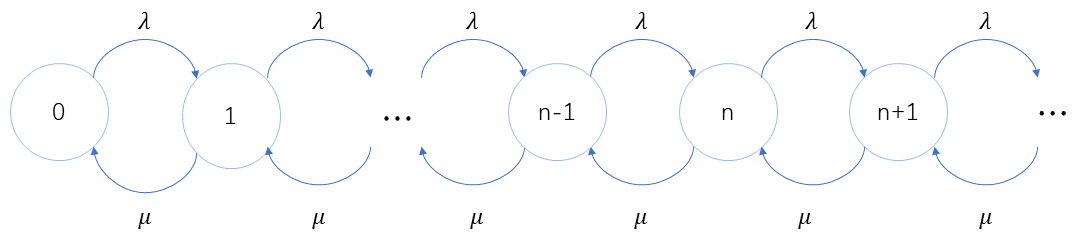
\includegraphics[width=.7\textwidth]{images/transform1.PNG}
    \caption{单通道状态转移图}
    \label{fig:transform1}
\end{figure}
\par 对于默认关门的情况,服务时间的均值$E(t_1)=2t_c+\frac{1}{\mu}$,
方差$Var(t_1)=0$
所以服务强度$\rho_1=2t_c\lambda_l+\frac{\lambda_l}{\mu}$,
由于将服务时间设置为确定值,所以直接使用Pollaczek-Khintchine公式进行求解。
得到理论上的平均队长$L_s=\rho_1+\frac{\rho_1^2}{2(1-\rho_1)}$。
\par 同理,对于默认开门的情况,服务时间是$t_2=t_r+t_{penal}$,
$t_{penal}$表示刷卡失败的惩罚时间,
随机变量$t_{penal}$可以用以下概率公式描述
\begin{equation}
    p(t_{penal})=
    \begin{cases}
        1-p_o,t_{penal}=T_{penal} \\
        p_o,t_{penal}=0
    \end{cases}
\end{equation}
其中$p_o$为开门成功率。$T_{penal}$为惩罚的具体时间大小。
这里的$t_r$与$t_{penal}$是相互独立的,因为后者是否存在仅仅取决于是否刷卡失败,
而这对随机服务时间,即刷卡时间与经过时间,没有任何影响。从而得到总服务时间的期望与方差如下:
\begin{equation}
    \begin{aligned}
        E(t_2) &=\frac{1}{\mu}+(1-p_o)T_{penal} \\
        Var(t_2)&=\frac{1}{\mu^2}+p_o(1-p_o)T_{penal}^2
    \end{aligned}
\end{equation}

所以服务强度$\rho_2=\lambda_l (1-p_o)T_{penal}+\frac{\lambda_l}{\mu}$,
直接运用Pollaczek-Khintchine公式得到理论上的平均队长
$L_s=\rho_2+\frac{\rho_2^2+\lambda^2/\mu^2+\lambda^2 p_o(1-p_o)T_{penal}^2}{2(1-\rho_2)}$
\par 最后将两者比较,得到两种服务方式的平均队长的比值
\begin{equation}
    \begin{aligned}
        \frac{L_{s1}}{L_{s2}}&=\frac{\rho_1+\frac{\rho_1^2}{2(1-\rho_1)}}{\rho_2+\frac{\rho_2^2+\lambda_l^2/\mu^2+\lambda_l^2 p_o(1-p_o)T_{penal}^2}{2(1-\rho_2)}} \\
        &=\frac{(2\rho_1-\rho_1^2)(1-\rho_2)}{(1-\rho_1)[2\rho_2-\rho_2^2+\lambda_l^2/\mu^2+\lambda_l^2 p_o(1-p_o)T_{penal}^2]}
    \end{aligned}
\end{equation}
其中$\rho_1=2t_c\lambda_l+\frac{\lambda_l}{\mu}$,
$\rho_2=\lambda_l (1-p_o)T_{penal}+\frac{\lambda_l}{\mu}$

接下来对结果进行简单的讨论:
\begin{itemize}
    \item 对于服务强度,$\rho_1-\rho_2=\lambda_l(2t_c-(1-p_o)T_{penal})$,
    由于$p_o$是一个很大的值,一般在0.9以上,所以默认关门的服务强度
    比默认关门要大得多,即在人流相同的条件下,默认开门的通行压力要更小。
    \item 对于这个公式,给出我们接下来数值时使用的参数,代入公式进行计算,
    具体取值如下:$t_c=0.5$,$\mu=1$,$p_o=0.9$,$T_{penal}=1$,$\lambda_l=0.2$,
    则$\rho_1=0.4,\rho_2=0.22$,从而$L_{s1}=\frac{3.2}{6},L_{s2}=0.278,\frac{L_{s1}}{L_{s2}}=1.9>1$。
    所以一般默认开门的平均队长是默认关门平均队长的0.52倍。
    也可以根据Little法则算出对应的等待时间比值,与平均队长的比值是一致的。
\end{itemize}

\subsubsection{模型建立}
\par 将校门前的道路网格化,假设行人占据一个网格、自行车占据两个网格。
根据假设,自行车在通过校门的时候会下车推行,
从而行人和自行车在门前的前进速度可以认为相同,设为$1m/s$。
对排队人群进行离散模拟,在每个模拟时间段内,如果行人或自行车前方空格
没有被占用,则前进一格。根据这样的模拟规则,将一个网格的长度设为$1m$。
\par 考虑单通行道的情况,模型可视化展示在图\ref{fig:one-lane-model}中。
\begin{figure}[ht]
    \centering
    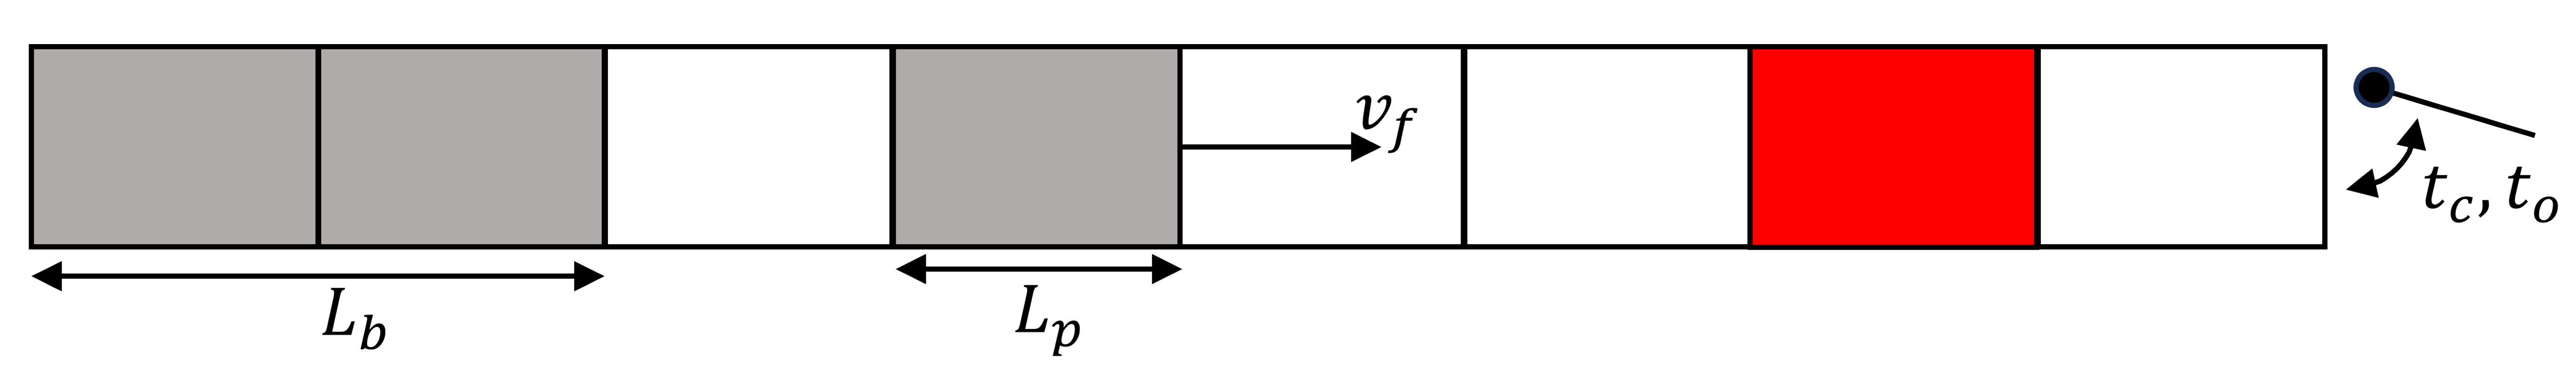
\includegraphics[width=0.6\textwidth]{images/cellular_automata_1_lane.png}
    \caption{单通行道模型可视化,其中灰色块表示网格被占用,红色块表示
    该通行者会刷卡失败(或没有校园卡),图中最右部分为校门}
    \label{fig:one-lane-model}
\end{figure}
\newline 其中:
\begin{itemize}
    \item $L_p, L_b$分别表示行人和自行车占用的网格长度
    \item $v_f$表示行人和自行车的前进速度
    \item $t_o, t_c$分别表示校门的开关时间,考虑实际情况,认为$t_c=t_o$
    \item $t_g,t_p$(图中未标注)分别为刷卡时间和通过时间,在确定性模型中
    两者视为定值
\end{itemize}
人和自行车均在道路最左边生成,道路有最大长度,当道路最左侧已经被占用时,
不再生成人。认为人的生成过程是一个泊松过程,对于高人流量和低人流量的时间段
泊松过程的参数取值不同。
\par 刷卡进校过程的拆分及两种开门方式的不同展示在图\ref{fig:process-entering-gate}中。
\begin{figure}[ht]    
    \centering
    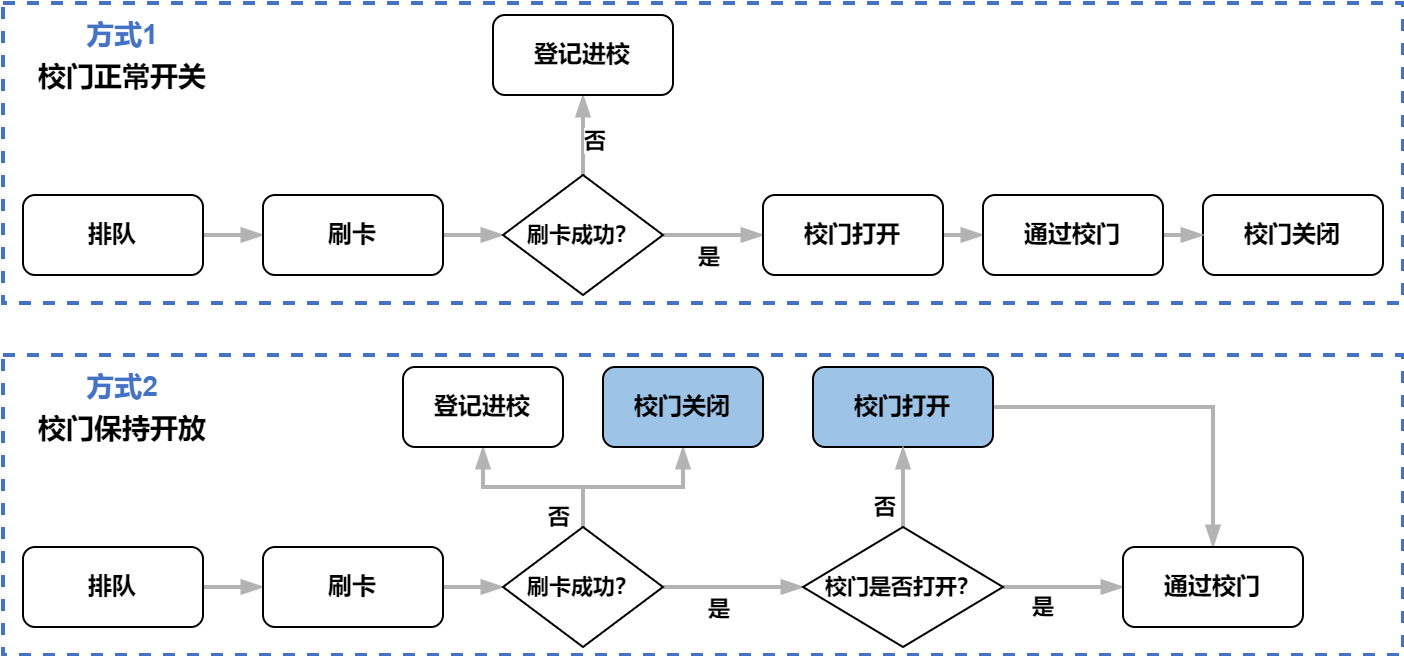
\includegraphics[width=.7\textwidth]{images/enter_gate_process.png}
    \caption{刷卡进校过程及两种校门开关方式的异同}
    \label{fig:process-entering-gate}
\end{figure}
在刷卡进校时,对于两种方法做相应的时间消耗分析:
\begin{itemize}
    \item 门保持开放:
    \begin{itemize}
        \item 如果刷卡成功,直接通过校门,需要的时间即为通过校门的时间加上
        刷卡识别的时间$t_p+t_g$。如果上一个人刷卡失败,该时间变为$t_g+t_o+t_p$。
        \item 如果刷卡失败,需要等待门关闭。根据实际生活经验,刷卡失败
        的个体在刷卡过程中一般花费时间也较长(例如询问在哪里刷身份证),同时
        刷卡失败之后,一般要离开队伍,然后登记入校。
        将这两个过程中时间的消耗合计为
        $t_{penal}$,从而刷卡失败消耗的时间为刷卡时间、等待门关闭的时间和
        离开队伍的时间加和$t_g+t_c+t_{penal}$。
    \end{itemize}
    \item 门正常开关:
    \begin{itemize}
        \item 如果刷卡成功,等待门开放后通过校门,下一个在队伍中的人等待门
        关闭后继续刷卡通过。从而一个人需要的时间为$t_g+t_o+t_p+t_c$。
        \item 如果刷卡失败,需要离开队伍。门正常开关时,不用等待门关闭,
        从而所需时间为$t_g+t_{penal}$。
    \end{itemize}
\end{itemize}

\subsubsection{数值模拟}
模拟的时间步长$t^*$取为$0.5s$,根据实际生活经验,约定开门的时间$t_o=t^*$、
行人的刷卡时间$t_g=t^*$、通过时间$t_p=t^*$、门关上的时间$t_c=t_o=t^*$。
如果刷卡失败,耽误的时间$t_{penal}=2t^*$。根据模型分析:
\begin{itemize}
    \item 门保持开放:
    \begin{itemize}
        \item 刷卡成功:耗时$t_p+t_g=2t^*$。
        \item 刷卡失败:耗时$t_g+t_c+t_{penal}=4t^*$。
    \end{itemize}
    \item 门正常开关:
    \begin{itemize}
        \item 刷卡成功:耗时$t_g+t_o+t_p+t_c=4t^*$。
        \item 刷卡失败:耗时$t_g+t_{penal}=3t^*$
    \end{itemize}
\end{itemize}
设置好以上参数以后,进行10000次模拟,每隔4个时间步长$t^*$取样一次,
设置队列容量为40,如果在模拟过程中,队列长度很少达到40,则表示符合队列容量无穷大的假设。
\par 数值模拟结果展示在图\ref{fig:queue-length-time}中,定性观察到
红色曲线几乎都在蓝色曲线上方,从而默认开门模式的队伍平均长度较短,即通行效率较高。
\par 为了定量描述两个模式效率的差距,绘制两模式队长比值-时间曲线在图\ref{fig:length-ratio-time-curve}中,
即$\frac{L_{s1}}{L_{s2}}-t$的关系。这个比值是通过对10000次取样的
队长取平均得到的平均队长,从而能够使得队长的比值趋于稳定。通过观察图像
与定量的数值分析,根据统计学知识,按照置信度为$\alpha=0.90$,计算得到
对应置信区间[0.4516,0.4526]。而上文中理论计算得到的比值为0.52,
可以得出两种模式下,理论分析的定性结论与实验一致,但定量结果略有偏差,这可能由于
理论推导中使用的是队伍极限情况的数据,但是数值模拟的时间长度是有限的。
\begin{figure}
    \centering
    \begin{minipage}[c]{0.45\textwidth}
        \centering
        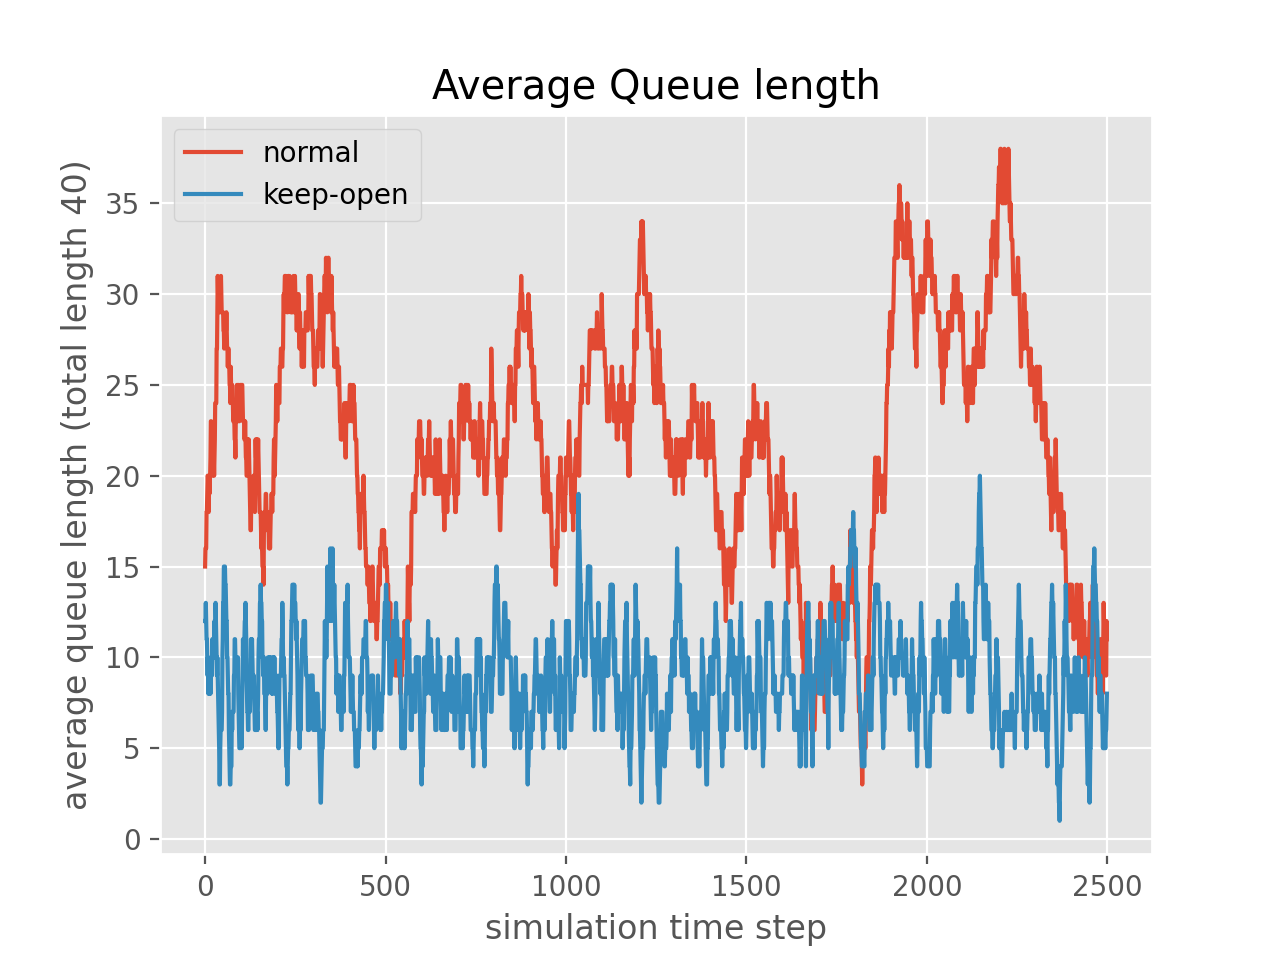
\includegraphics[width=1.\textwidth]{images/队长-时间曲线.png}
        \subcaption{单通道确定性模型队长-时间曲线,其中红色线表示正常开门方式,蓝色线表示校门保持
        开放}
        \label{fig:queue-length-time}
    \end{minipage}
    \begin{minipage}[c]{0.45\textwidth}
        \centering
        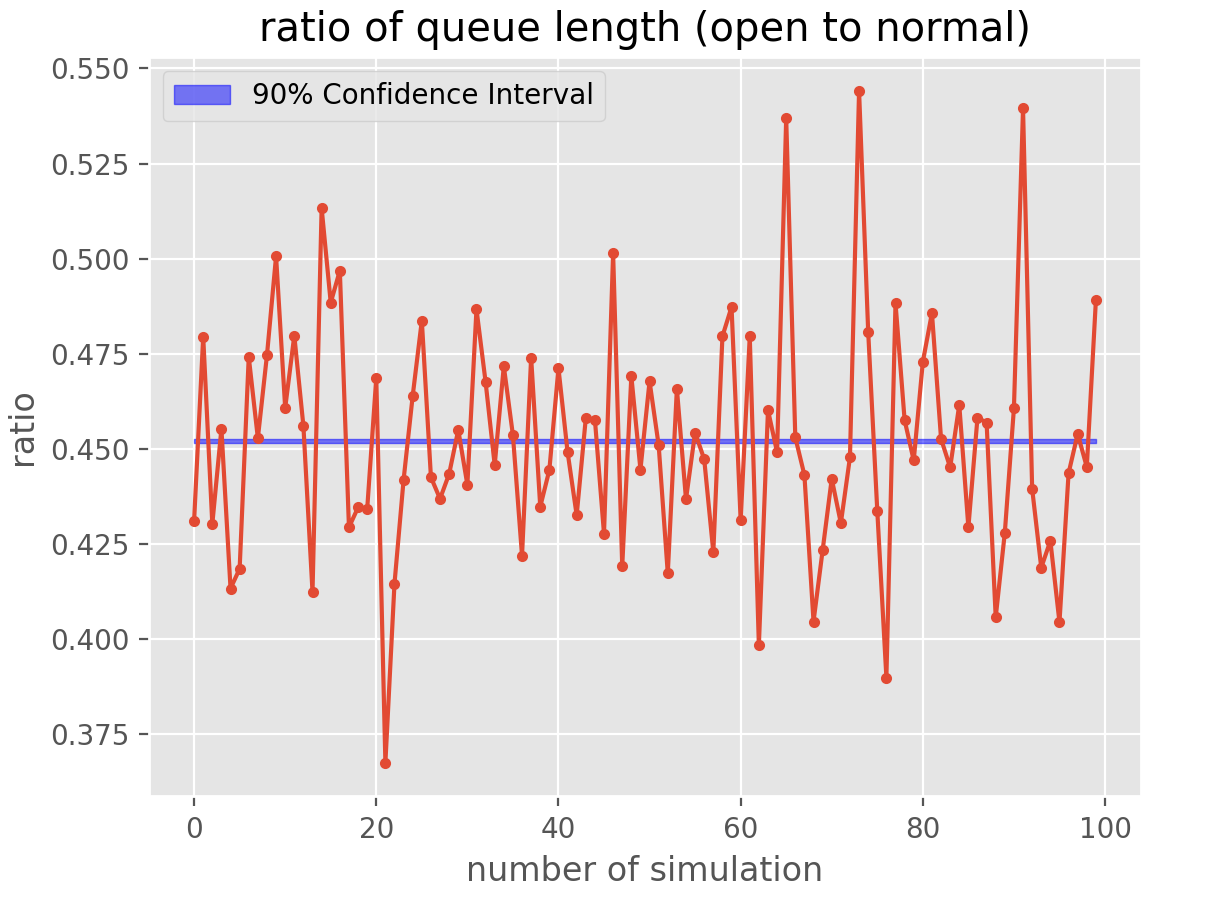
\includegraphics[width=1.\textwidth]{images/队长比例-时间曲线.png}
        \subcaption{单通道确定性模型两模式队长比值-时间曲线}
        \label{fig:length-ratio-time-curve}
    \end{minipage}
    \caption{单通道确定性模型数值模拟}
    \label{fig:one-lane-numerical-result}
\end{figure}
\par 在图\ref{fig:queue-length-time}中观察到,在正常开门的情况下,
队伍人数在到达一个极值后存在直线下降的情况,这与生活经验有差别。
出现这种情况可能由于,模型中规定如果道路已经被填满则不会再生成人,这与实际
情况是不一致的。所以在之后的模型中,用一个``缓冲区''
来存储当道路填满时生成的人,更好地拟合实际情况。
\subsection{单通道随机性模型}
\subsubsection{理论分析}
考虑非高峰期的情况下,使用一个参数为$\lambda_{l}$的泊松过程来表示顾客源,
使用负指数分布的随机服务时长,即$M/G/1/\infty/\infty/FCFS$模型。
其中使用的是G而不是M是因为总的服务时长$t_{all}=2t_{c}+t_{r}$,是一个
符合负指数分布的变量加上一个常量,并不是严格的负指数分布,所以用一般分布G表示。
\par 对本模型的求解,主要按照按模型1的求解方法,先建立对应稳态之间的差分方程:
\begin{equation}
    \begin{aligned}
        \lambda P_{n-1}(t)+\frac{\mu}{2t_c\mu+1} P_{n+1}(t)-(\lambda+\frac{\mu}{2t_c\mu+1} )P_n(t)& =0,n\geq 1 \\
        -\lambda P_{0}+\frac{\mu}{2t_c\mu+1} P_{1}&=0
    \end{aligned}
\end{equation}
求解这个差分方程可以得到对应状态的概率
\begin{equation}
    \begin{aligned}
        P_0 &=1-\rho \\
        P_n &=(1-\rho)\rho^n,n\geq1
    \end{aligned}
\end{equation}
其中的$\rho=2\lambda t_c+\frac{\lambda}{\mu}$,它的物理意义为服务强度。
随后,通过与模型1类似的方法可以得到对应状态转移关系。
图\ref{fig:transform2}中展示了不同状态转移关系。
\begin{figure}[ht]
    \centering
    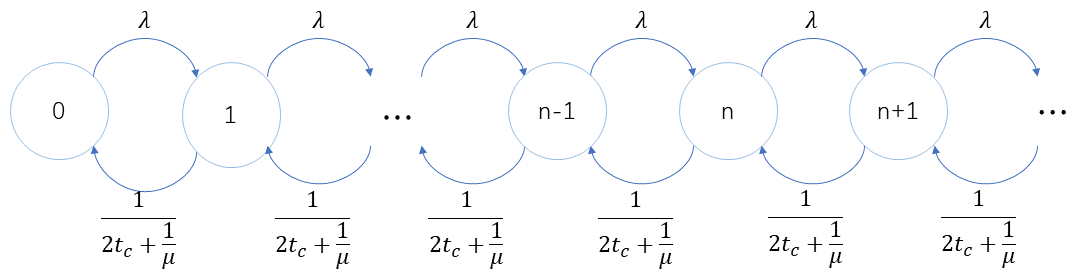
\includegraphics[width=.6\textwidth]{images/transform2.PNG}
    \caption{随机模型单通道状态转移图}
    \label{fig:transform2}
\end{figure}
\par 对于默认关门的情况,服务时间是$t_1=2t_c+\frac{1}{\mu}$,
所以服务强度$\rho_1=2t_c\lambda_l+\frac{\lambda_l}{\mu}$,
得到理论上的平均队长$L_s=\frac{\rho_1}{1-\rho_1}$。
\par 同理,对于默认开门的情况,服务时间是$t_2=t_r+t_{penal}$,
$t_{penal}$表示刷卡失败的惩罚时间,惩罚时间的建模与上一个模型一致。

其中$p_o$为开门成功率。$T_{penal}$为惩罚的具体时间大小。
这里的$t_r$与$t_{penal}$是相互独立的,因为后者是否存在仅仅取决于是否刷卡失败,
而这对随机服务时间,即刷卡时间与经过时间,没有任何影响。从而得到总服务时间的期望与方差如下:
\begin{equation}
    \begin{aligned}
        E(t_2) &=\frac{1}{\mu}+(1-p_o)T_{penal} \\
        Var(t_2)&=\frac{1}{\mu^2}+p_o(1-p_o)T_{penal}^2
    \end{aligned}
\end{equation}

所以服务强度$\rho_2=\lambda_l (1-p_o)T_{penal}+\frac{\lambda_l}{\mu}$,
直接运用Pollaczek-Khintchine公式得到理论上的平均队长
$L_s=\rho_2+\frac{\rho_2^2+\lambda^2/\mu^2+\lambda^2 p_o(1-p_o)T_{penal}^2}{2(1-\rho_2)}$
\par 最后将两者比较,得到两种服务方式的平均队长的比值
\begin{equation}
    \begin{aligned}
        \frac{L_{s1}}{L_{s2}}&=\frac{\frac{\rho_1}{1-\rho_1}}{\rho_2+\frac{\rho_2^2+\lambda_l^2/\mu^2+\lambda_l^2 p_o(1-p_o)T_{penal}^2}{2(1-\rho_2)}} \\
        &=\frac{2\rho_1(1-\rho_2)}{(1-\rho_1)[2\rho_2-\rho_2^2+\lambda_l^2/\mu^2+\lambda_l^2 p_o(1-p_o)T_{penal}^2]}
    \end{aligned}
\end{equation}
其中$\rho_1=2t_c\lambda_l+\frac{\lambda_l}{\mu}$,
$\rho_2=\lambda_l (1-p_o)T_{penal}+\frac{\lambda_l}{\mu}$
\par 对结果进行简单的讨论:
\begin{itemize}
    \item 对于服务强度,$\rho_1-\rho_2=\lambda_l(2t_c-(1-p_o)T_{penal})$,
    由于$p_o$是一个很大的值,一般在0.9以上,所以默认关门的服务强度
    比默认关门要大得多,即在人流相同的条件下,默认开门的通行压力要更小。
    \item 对于这个公式,给出我们接下来数值时使用的参数,代入公式进行计算,
    具体取值如下:$t_c=0.5$,$\mu=1$,$p_o=0.9$,$T_{penal}=1$,$\lambda_l=0.2$,
    则$\rho_1=0.4,\rho_2=0.22$,从而$L_{s1}=\frac{2}{3},L_{s2}=0.278,\frac{L_{s1}}{L_{s2}}=2.4>1$。
    所以一般默认开门的平均队长是默认关门平均队长的0.42倍。
    也可以根据Little法则算出对应的等待时间比值,与平均队长的比值是一致的。
\end{itemize}
\subsubsection{模型建立与求解}
在确定性模型中,刷卡时间和通行时间(之后统称为服务时间)认为是常数,
在实际情况中,服务时间往往会因为客户对象的不同而发生变化。
选择利用负指数分布刻画这种服务时间的不确定性,从而更好地刻画队伍的运动情况。
\par 由于负指数分布可能给出过大的服务时间值,在数值模拟时将负指数分布产生的
随机数限制在区间$[t^*, 6 t^*]$内,其中$t^*$为模拟的时间步长。
数值模拟过程中,参数取值为:
\begin{itemize}
    \item 道路长度为40
    \item 生成对象的过程服从$\lambda_l = 0.2$的泊松分布
    \item 对于生成的对象,是行人的概率为0.8,是自行车的概率为0.2
    \item 负指数分布的参数$\mu = 2t^*$
    \item 刷卡成功率为0.9
    \item 模拟次数为10000,每隔4次记录平均队长
\end{itemize}
同时在人的生成部分,采用一个缓冲区存储没有能够立刻进入队伍的人。
模拟得到平均队长的变化(30步移动平均)记录在图\ref{fig:average-length-with-exp}中。
\begin{figure}[ht]
    \centering
    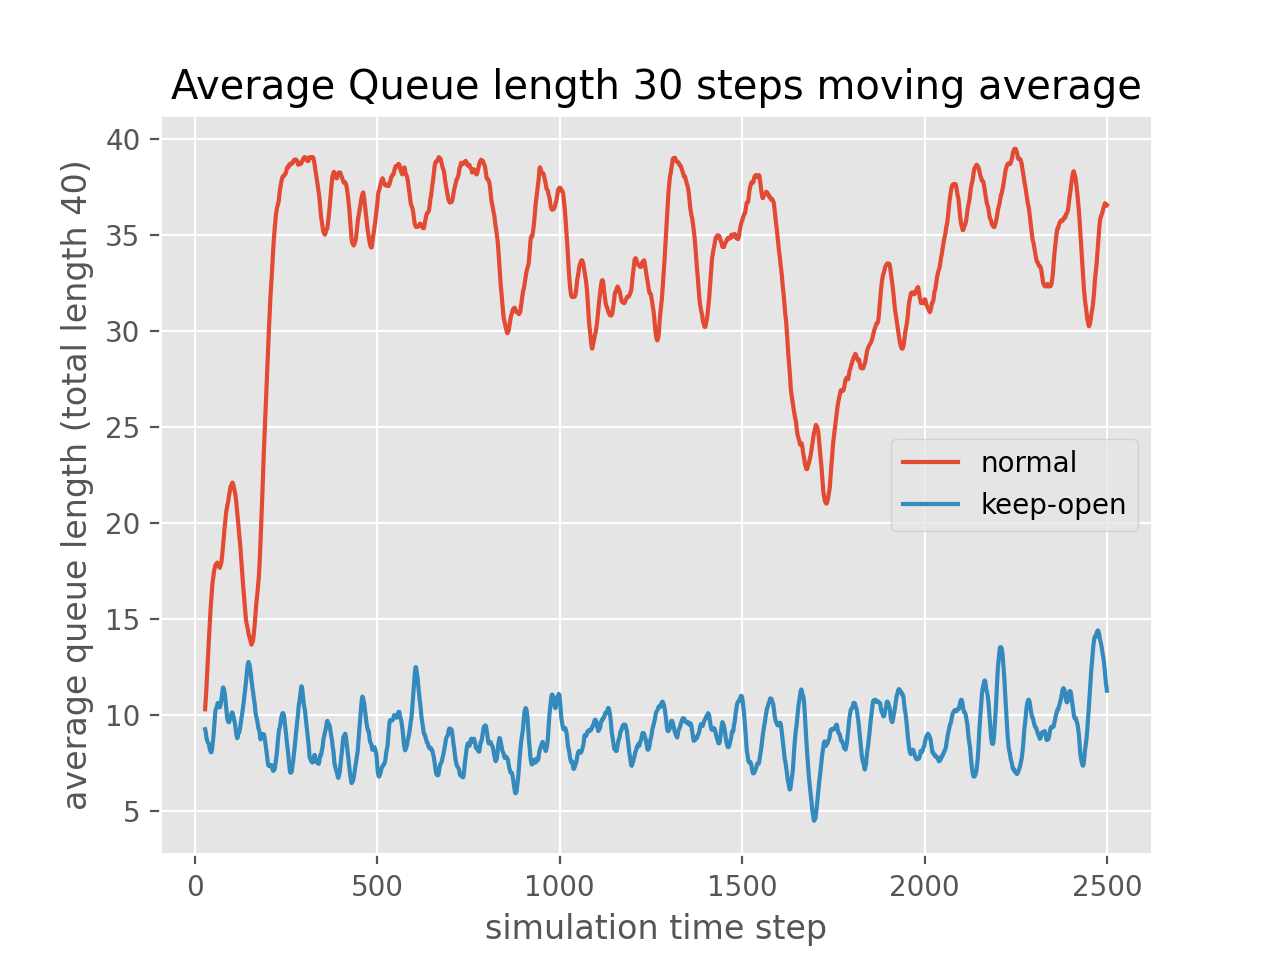
\includegraphics[width=.6\textwidth]{images/avg_queue_length_with_exp.png}
    \caption{服务时间满足负指数分布的平均队长,其中红线为校门的正常开关状态,蓝线
    为校门保持开放}
    \label{fig:average-length-with-exp}
\end{figure}
图\ref{fig:average-length-with-exp}相较图\ref{fig:queue-length-time}
少了很多人数直线下降的情况,说明缓冲区的选取更加符合实际。
观察到校门正常开放的队伍平均长度明显大于校门保持开放时的平均长度。
在遇到服务时间较长的情况时,由于不能换道,队伍很容易出现充满的情况,造成平均队长保持在
一个较大的值,此时门常开对于通行效率的优势体现的更为明显。
\par 刷卡成功率对于两种通行方式的效率有很大的影响,将成功率下调为0.4后,得到的
平均队长的比值(常开/正常)关于模拟次数的曲线展示在图\ref{fig:low-success-rate}中。
\begin{figure}[ht]
    \centering
    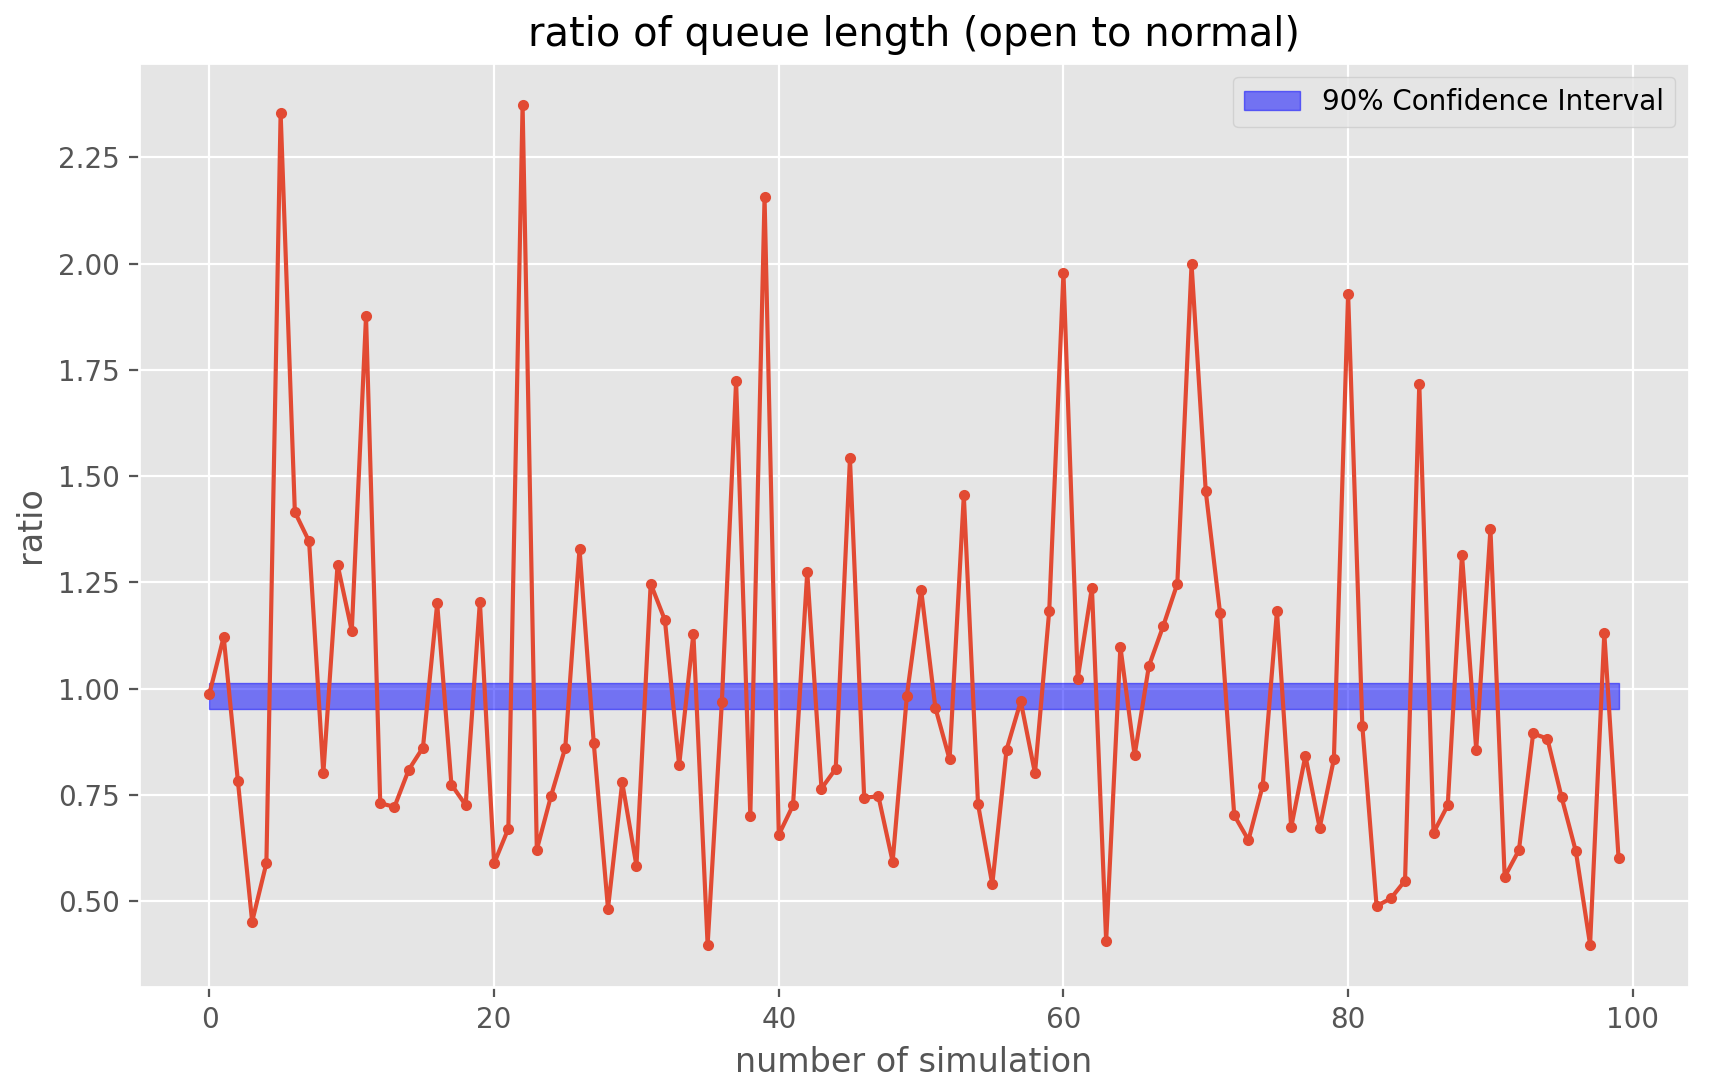
\includegraphics[width=.7\textwidth]{images/ratio_low_success_rate.png}
    \caption{成功率为0.4时的平均队长比值(常开/正常)与比例平均值90\%置信区间}
    \label{fig:low-success-rate}
\end{figure}
从图\ref{fig:low-success-rate}中明显观察到,比例均值的置信区间由之前的0.45上升到接近
1,说明两种方法在刷卡失败率较高时通行效率相差不大。但是如果进一步考虑安全性、便于管理性,
门正常开关在这种情况下好于门保持开放。
\subsection{多通道模型}
\subsubsection{理论分析}
考虑非高峰期与高峰期的情况下,使用参数为$\lambda_{l},\lambda_{h}$的泊松过程来表示顾客源,
使用负指数分布的随机服务时长,考虑多通道且允许相互转移的过程,这个相互转移的发生条件是:
假设人流自发流向长度最短的队伍,
即$M/G/3/C_{queue}/C_{source}/FCFS$模型。

设置服务站数c=3,这会影响到差分方程的建立与求解过程。

以下是不同状态转移关系:
\begin{figure}[ht]    
    \centering
    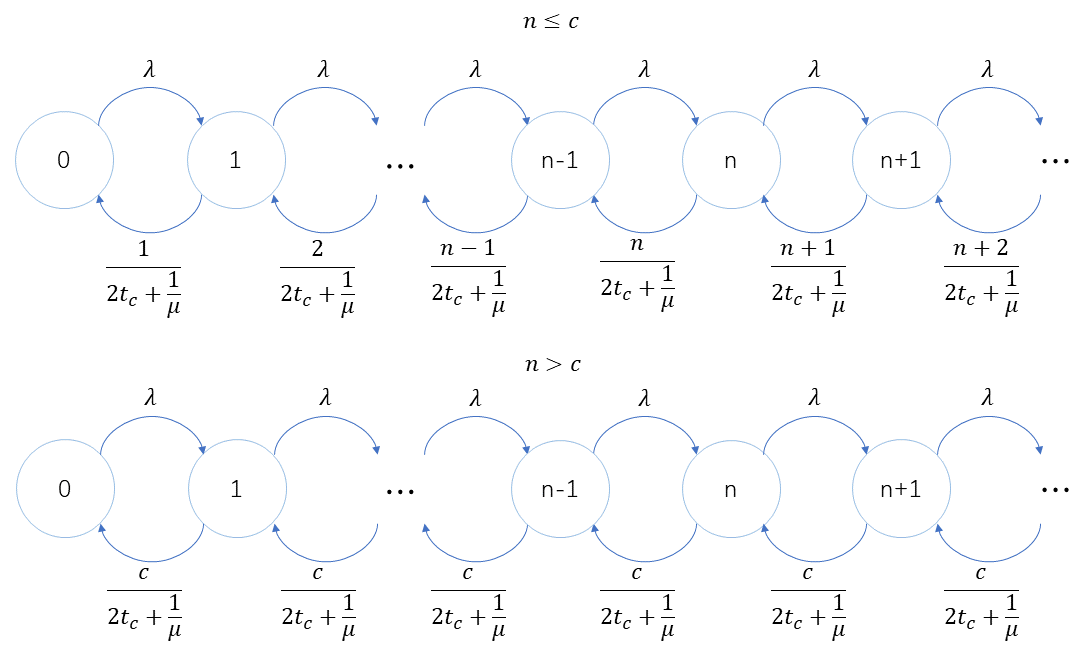
\includegraphics[width=.6\textwidth]{images/transform3.PNG}
    \caption{多通道状态转移图}
    \label{fig:transform3}
\end{figure}

对于非高峰期的多通道模型,
对应的差分方程模型如下:
\begin{equation}
    \begin{aligned}
        &\mu P_1=\lambda P_0 \\
        &(n+1)\mu P_{n+1}+\lambda P_{n-1}=(\lambda+n\mu)P_n, 1\leq n\leq c \\
        &c\mu P_{n+1}+\lambda P_{n-1}=(\lambda +c\mu )P_n, n>c
    \end{aligned}
\end{equation}

其中的$\rho=\frac{\lambda}{\mu}\geq 1$,否则队长会发散。
求解结果如下:
\begin{equation}
    \begin{aligned}
        &P_0=\Big[\sum_{k=0}^{c-1}\frac{1}{k!} \rho^k +\frac{1}{c!(1-\rho)}\cdot \rho^c \Big]^{-1} \\
        &P_n=
        \begin{cases}
            \frac{1}{n!}\rho^n P_0 \\
            \frac{1}{c!c^{n-c}}\rho^n P_0
        \end{cases}
    \end{aligned}
\end{equation}

从而求得平均对长$L_s=\frac{(c\rho)^c\rho}{c!(1-\rho)^2}P_0+\rho$

对于高峰期的多通道模型,
对应的差分方程模型如下:
\begin{equation}
    \begin{aligned}
        &\mu P_1=\lambda P_0 \\
        &(n+1)\mu P_{n+1}+\lambda P_{n-1}=(\lambda+n\mu)P_n, 1\leq n\leq c \\
        &c\mu P_{n+1}+\lambda P_{n-1}=(\lambda +c\mu )P_n, n>c
    \end{aligned}
\end{equation}

其中的$\rho=\frac{\lambda}{\mu}\geq 1$,否则队长会发散。
由于队列的容量有限,用$N=C_{queue}$,所以有限制$\sum_{k=0}^{N}P_k=1$
求解结果如下:
\begin{equation}
    \begin{aligned}
        &P_0=\Big[\sum_{k=0}^{c}\frac{1}{k!} (c\rho)^k +\frac{c^c\rho (\rho^c-\rho^N)}{c!(1-\rho)} \Big]^{-1} \\
        &P_n=
        \begin{cases}
            \frac{1}{n!}(c\rho)^n P_0 \\
            \frac{c^c}{c!}\rho^n P_0
        \end{cases}
    \end{aligned}
\end{equation}

从而求得平均对长$L_s=\frac{(c\rho)^c\rho}{c!(1-\rho)^2}P_0[1-\rho^{N-c}-(N-c)\rho^{N-c}(1-\rho)]+c\rho (1-\rho)$
多通道模型的非高峰期与高峰期理论求解完毕。

\subsubsection{模型建立与求解}
\par 实际情况中,往往有多条入校通道。相较于单通道,多通道的引入,使得
行人和自行车在条件允许时,可以选择更换通道,从而更快地通过校门。
在实际情况中,如果当前通道有人刷卡失败,行人会有一定的概率更换通道。
在模型中,规定:
\begin{itemize}
    \item 当相邻的网格没有被占用
    \item 当换到的网格正后方网格没有被占用时
\end{itemize}
行人将以$p_s=0.5$的概率换到相邻的网格。模拟过程中取通道数量为3,模型可视化
展示在图\ref{fig:3-lanes-model}中。
\begin{figure}[ht]
    \centering
    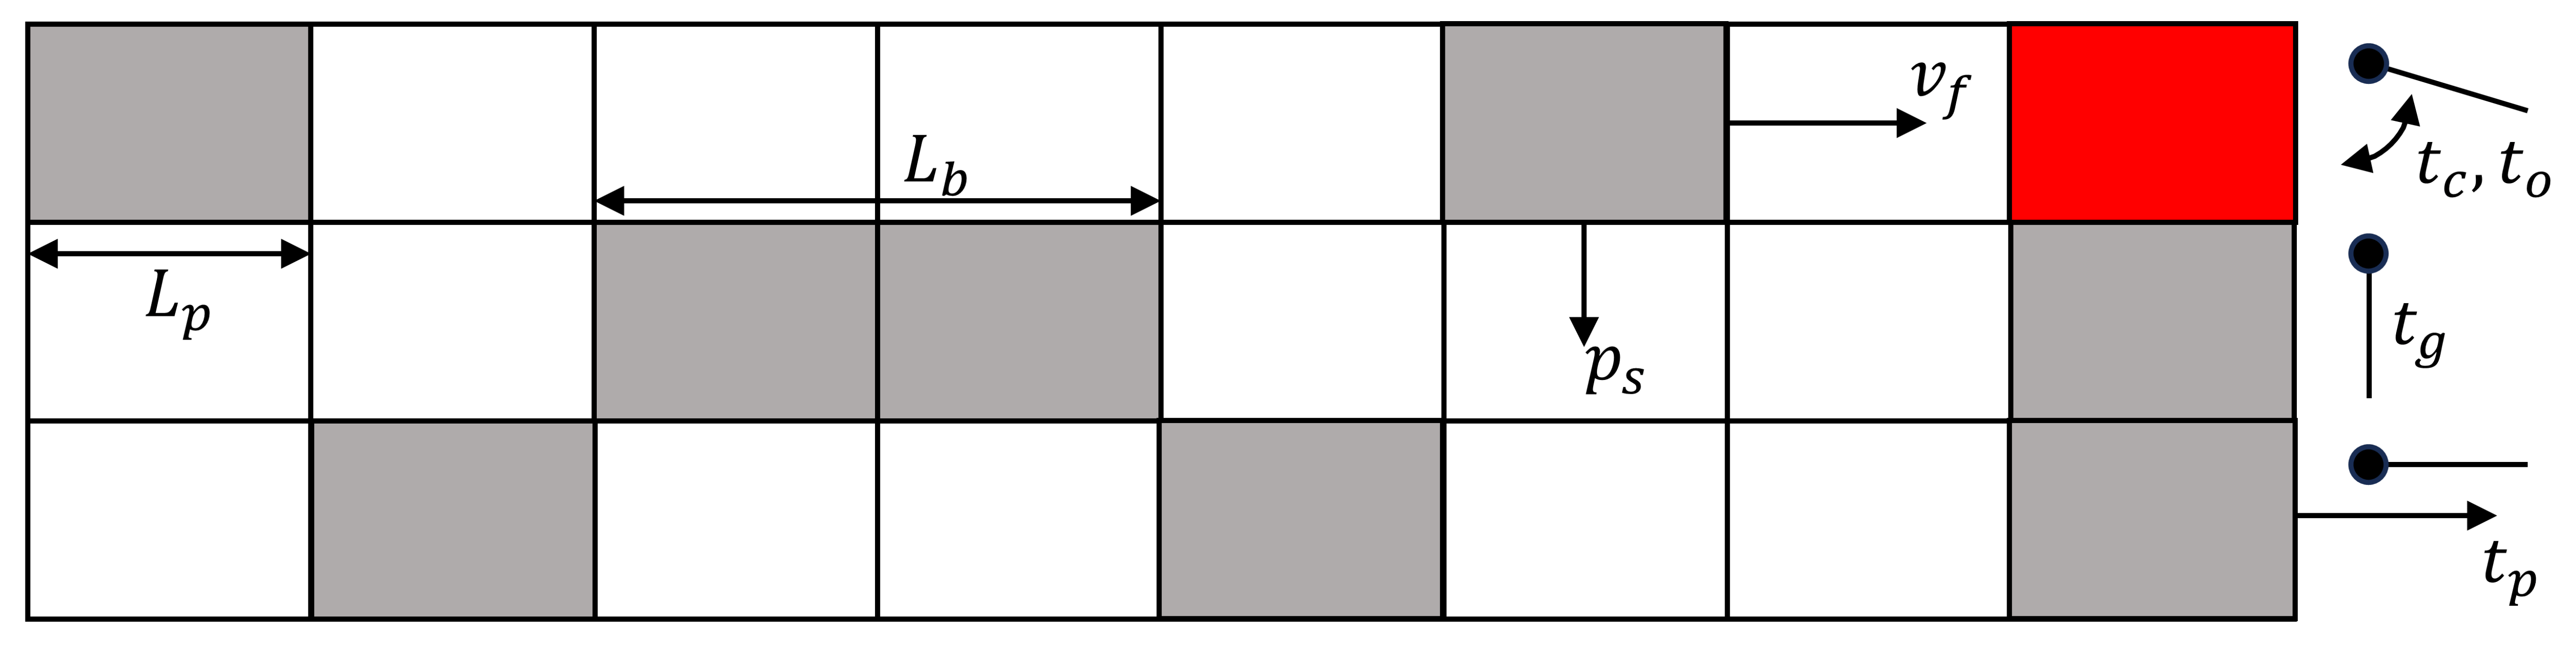
\includegraphics[width=.7\textwidth]{images/cellular_automata_3_lanes.png}
    \caption{三通道模型示意图}
    \label{fig:3-lanes-model}
\end{figure}
\par 对比多通道和单通道模型,选取1000个模拟步长,成功率0.9,分别模拟
非高峰期($\lambda_l = 0.2$)和高峰期($\lambda_h = 0.4$)的结果
展示在图\ref{fig:model-three-result}中。
\begin{figure}[ht]
    \centering
    \begin{minipage}[c]{0.45\textwidth}
        \centering
        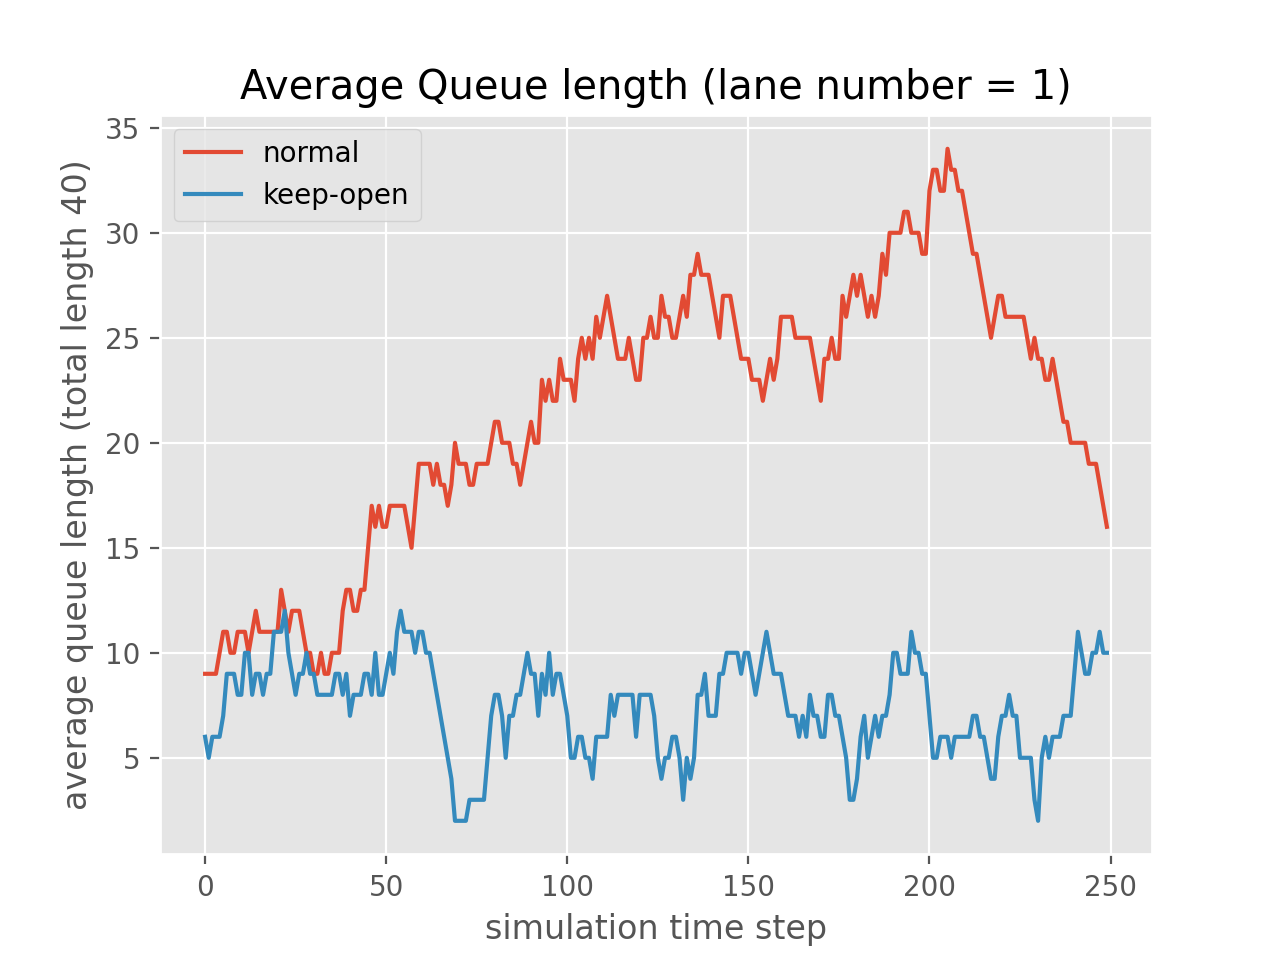
\includegraphics[width=.9\textwidth]{images/queue_length_poisson_one_lane_low.png}
        \subcaption{单通道随机模型低人流量时平均队长变化}
        \label{fig:one-lane-low-poisson}
    \end{minipage}
    \begin{minipage}[c]{0.45\textwidth}
        \centering
        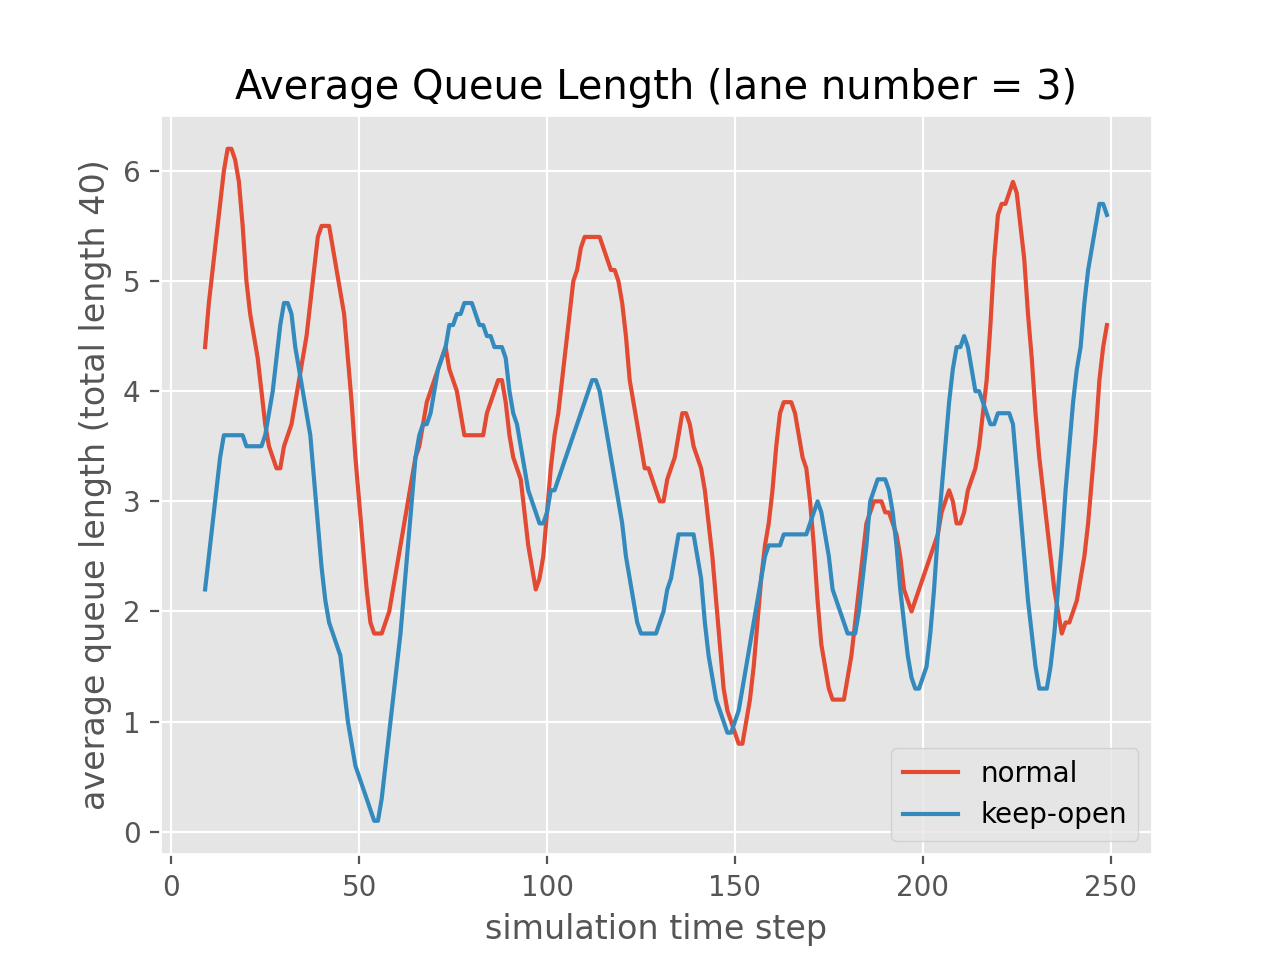
\includegraphics[width=.9\textwidth]{images/queue_length_poisson_three_lane_low_ma.png}
        \subcaption{多通道随机模型低人流量时平均队长变化(10步滑动平均)}
        \label{fig:three-lane-low-poisson}
    \end{minipage}
    \begin{minipage}[c]{0.45\textwidth}
        \centering
        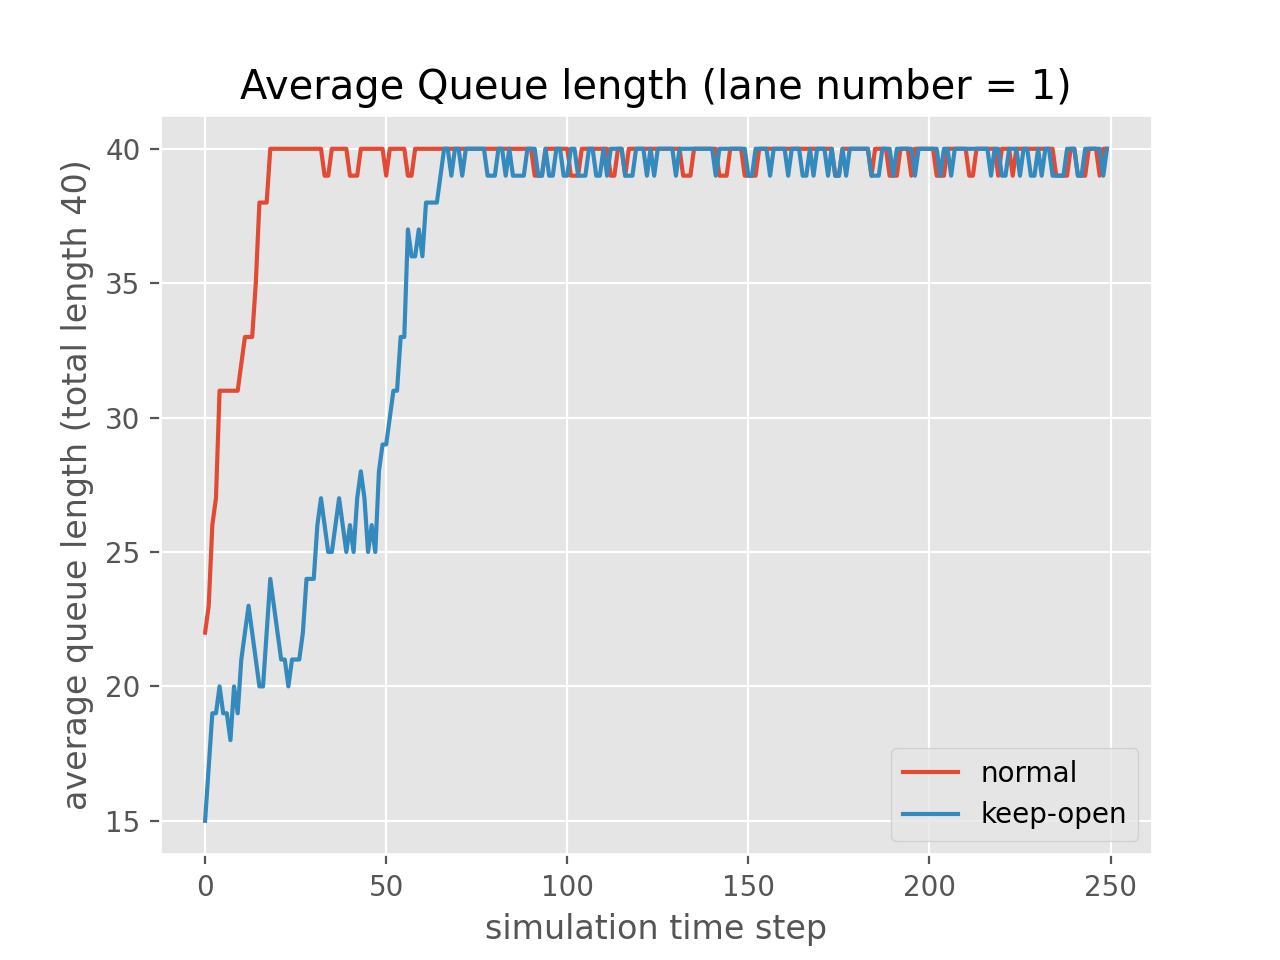
\includegraphics[width=.9\textwidth]{images/queue_length_poisson_one_lane_high.png}
        \subcaption{单通道随机模型高人流量时平均队长变化}
        \label{fig:one-lane-high-poisson}
    \end{minipage}
    \begin{minipage}[c]{0.45\textwidth}
        \centering
        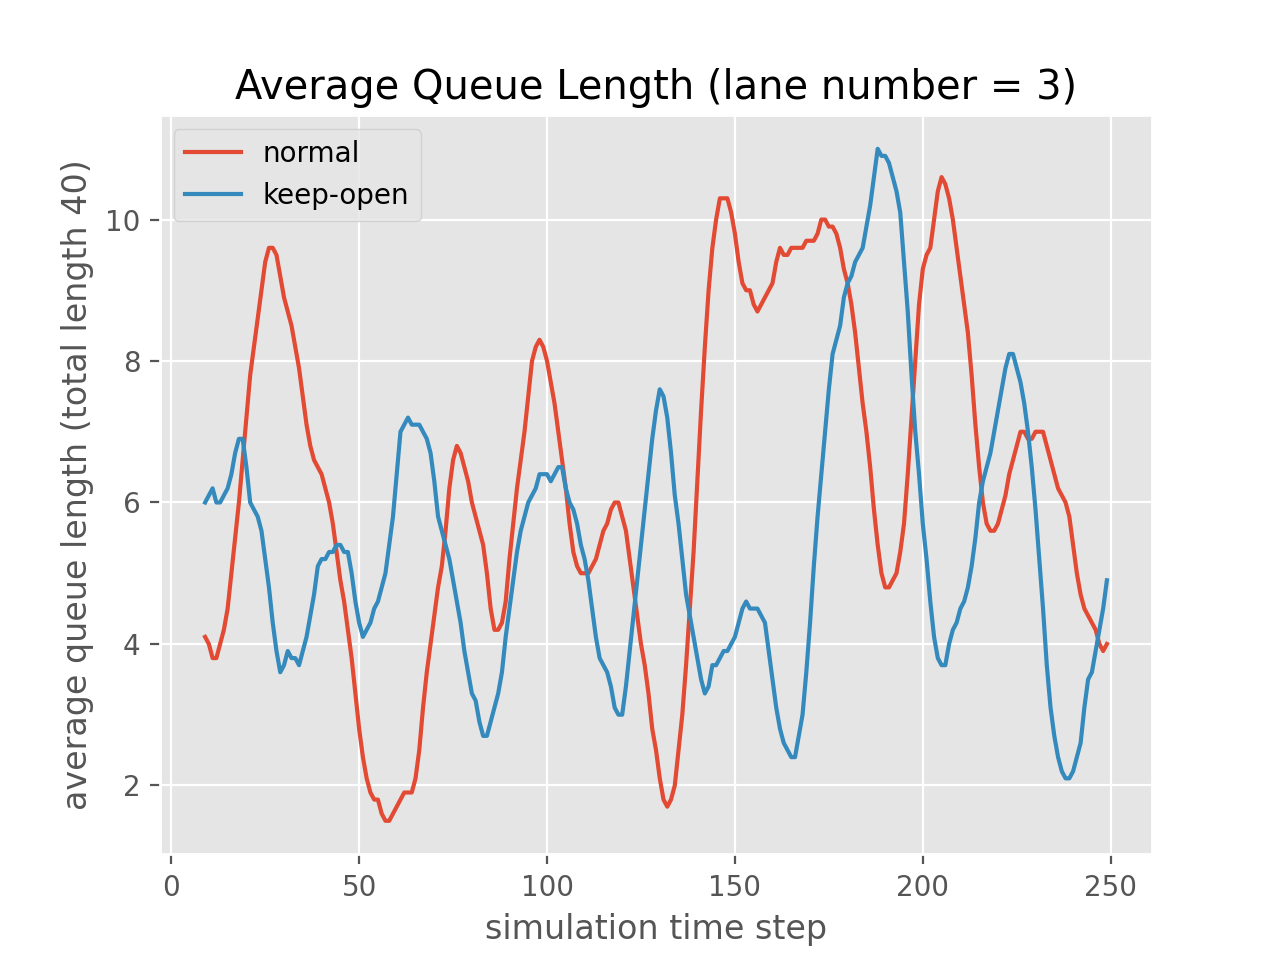
\includegraphics[width=.9\textwidth]{images/queue_length_poisson_three_lane_high_ma.png}
        \subcaption{多通道随机模型低人流量时平均队长变化(10步滑动平均)}
        \label{fig:three-lane-high-poisson}
    \end{minipage}
    \caption{多通道与单通道随机模型在高低人流量情况下平均队长对比}
    \label{fig:model-three-result}
\end{figure}
\subsection{基于数值模拟结果的通行方式建议}
\par 在非高峰期,根据模型结果,默认关门的平均队长比大约是默认开门的两倍,
通行效率显著低于后者,几乎没有可比性。在高峰期且刷卡失败率较高时,
两种通行模式的的平均队长之比趋近于1,表明两者的效率相近。而这时,
默认关门比默认开门的安全性大大提高。所以在人流较大且刷卡失败率
高的情况下,应当使用默认关门的模式。
\par 就同济大学而言,在特殊时期,例如樱花季、部分法定假期等,
人流量显著提高,且主要通行人员的身份从学生转为游客,刷卡成功率大大降低,
而且安全性也有所降低。这时使用默认关门的模式,在通行效率上没有太大的影响,
而在安全性上得到提高。而在平常时期,出入主体为学生,可以使用默认开门
的模式,提高通行效率。
\par 除此以外,此模式还可以推广到其他出入系统,如地铁站。
地铁站对于安全性的要求较高,且在客流量较大时还需要考虑管理问题,从而
需要综合考虑人流量、通行人主要成分、通行时间段等因素,
综合判断通行效率与安全性,给出对应开门方式。
\section{模型评价}
\subsection{模型优缺点}
\subsubsection{模型优点}
\begin{itemize}
    \item 使用排队论中的经典理论,先得到理论结果,对两种模式做出定性与定量的比较。
    \item 使用元胞自动机模型对排队-通行的过程进行精细模拟,
    考虑不同时间段(非高峰期与高峰期),不同形式(单通道与多通道)。
    \item 使用蒙特卡洛法进行模拟,对结果进行统计分析,从而验证理论解的正确性。
    \item 对排队过程进行可视化分析,使得排队过程得以展现,从而直观地观察到不同开门模式的差异性。
\end{itemize}
\subsubsection{模型缺点}
\begin{itemize}
    \item 使用的是排队论中的基础模型,虽然经分析可知模型可以基本符合
    改场景的情况,但过于理想化的模型在定量描述方面有一定缺陷。
    \item 在统计学意义上,样本数量不够大,如果增加模拟次数可以使结果更加准确。
    \item 理论解过于理想化,求解的结果单一,容易与实验结果发生偏差,对于这种
    随机服务系统,应该按照其随机性的规律,确定结果范围,防止出现过大偏差。
\end{itemize}
\subsection{改进方向}
\begin{itemize}
    \item 实地调研,统计得到对应参数的参考值,获取各项参数的统计规律。
    \item 深入研究排队论,选择更为符合实际统计规律的概率模型,提高定量分析的准确度。
    \item 将模型推广到更多使用场景,如地铁站出入口,对于不同场景建立恰当的
    排队论模型与元胞自动机模型,进行理论分析与数值模拟。
\end{itemize}

% \begin{thebibliography}{9}%宽度9
% \bibitem[1]{20120118}
% 刘延柱.
% \newblock 关于摩擦碰撞的Kane难题\allowbreak[J/OL].
% \newblock 力学与实践, 2012, 34\penalty0 (1):\penalty0 91-94.
% \newblock \url{https://lxsj.cstam.org.cn/cn/article/doi/10.6052/1000-0879-20120118}.

% \bibitem[2]{doi:10.1098/rspa.2013.0497}
% COHEN~C, DARBOIS-TEXIER~B, DUPEUX~G, et~al.
% \newblock The aerodynamic wall\allowbreak[J/OL].
% \newblock Proceedings of the Royal Society A: Mathematical, Physical and Engineering Sciences, 2014, 470\penalty0 (2161):\penalty0 20130497.
% \newblock \url{https://royalsocietypublishing.org/doi/abs/10.1098/rspa.2013.0497}.

% \bibitem[3]{20130314-2}
% 刘延柱.
% \newblock 再论Kane难题\allowbreak[J/OL].
% \newblock 力学与实践, 2013, 35\penalty0 (3):\penalty0 77-79.
% \newblock \url{https://lxsj.cstam.org.cn/cn/article/doi/10.6052/1000-0879-12-170}.
% \end{thebibliography}

\end{document}